
\subsubsection{Overview}

This component is the interface for the Refbox. It handles the communication between the Refbox and the robotinos. Its functionality is very important, since communication to the referee box is essential to receive game instructions and report sensed information to gain points. If you need a full understanding of the communication patterns, it is recommended to read also the referee box manual located at \url{ http://www.robocup-logistics.org/refbox}. It describes the used protobuf (\url{https://developers.google.com/protocol-buffers}) messages in a detailed way. In the current state, the component covers most of the use cases needed for the Robocup competition.


\subsubsection{Situation in 2016}

In the old version of the code, the RefBox Server component was not used to send back information about detected MPS \cite{BOK}. So, there was no complete communication with InstructionPlaner and Refbox. There was not Refbox installed in the laboratory. 


\subsubsection{Situation in 2017}

About the Refbox server component, some new objects need to be handled (new zones, new MPS) that's why some communication objects have been added. Getting from the Refbox the team color and current game phase is working and tested. Send color and phase to InstructionPlaner component is also working. The detection of the maintenance phase is now possible. Send MPS information like zones, orientation from Refbox server to Refbox is working. The Refbox adds successfully points for good MPS reports and remove points for wrong MPS reports. It is necessary to modify the following parameters: the \textbf{HostIP} which is the IP address of the referee box, the \textbf{Name} which represent the name of the robotino (this name will be listed on the referee box GUI), the \textbf{Number} which is the (jersey) number of the robotino (this number will be listed at the referee box GUI) and the \textbf{Cryptokey} which is the key used for the encrypted team channel.\\

\subsubsection{Classes}

There are several classes in the Refbox Server component. Each class will be described here. Reading the source code at the same time is recommended.\\

\begin{figure}[!h]
\centering
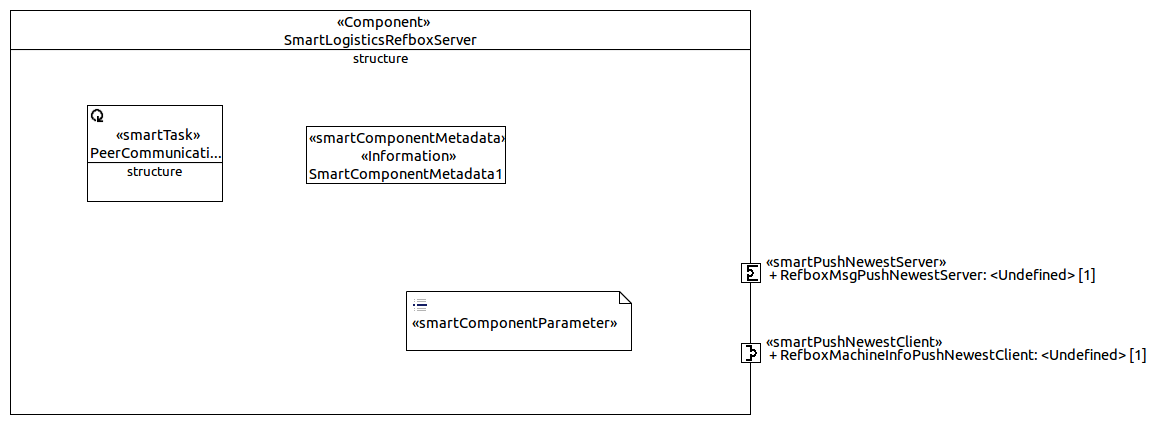
\includegraphics[width=\linewidth]{pic/component_refbox_server.png}
\caption{Model of Refbox server}
\label{fig:modelRefboxServer}
\end{figure}

First, the \textbf{RefboxPeer} class owns the instances of protobuf peers. One peer is created for the team channel and another one for the public channel. The peers are used to receive and send protobuf messages via the corresponding channels. Note that our robots never send via the public channel, but only listen to it. All used protobuf messages must be registered in the peer’s message register. To handle all received messages, the peers are connected to a signal handler, which is represented by the class \textbf{CommunicationHandler}. \\

Next, the \textbf{CommunicationHandler} class permit to trigger the handle message method when a message is received from a connected peer. Depending on the type of the message, a specific evaluation method of the \textbf{MessageEvaluator} class is called to decode the message.\\

Then, the \textbf{MessageEvaluator} class has an overloaded method named evaluate which applies for any kind of message type. However, not all of the overloaded variants have been implemented so far. Until now, only the relevant message types needed for the exploration phase are completely realised (GameState and ExplorationInfo). Each variant is supposed to read the protobuf message and to extract the most important information into the internal communication objects of type CommRefbox. Those are used to pass the relevant information to the instruction planner component. In the production phase, the evaluate method for the orderInfo message has to be developed.\\

Next the \textbf{ConnectionMaintenance} class has a task which sends a beacon signal every two seconds via the team peer. This is the periodic heartbeat signal to the referee box, which makes the referee box aware of the robots’ presence. Therefore, also some information about the robot is contained in the message, such as its name, team name and number.\\

Finally, the \textbf{PeerCommunication} class is the component’s smartTask of the SmartSoft environment. This means this is the loop construct which will be run as long as the component is active. At the current state, it does nothing more than sending new registered information about the gamestate or explorationinfo messages to the instruction planner via the push server.\\

\begin{figure}[!h]
\centering
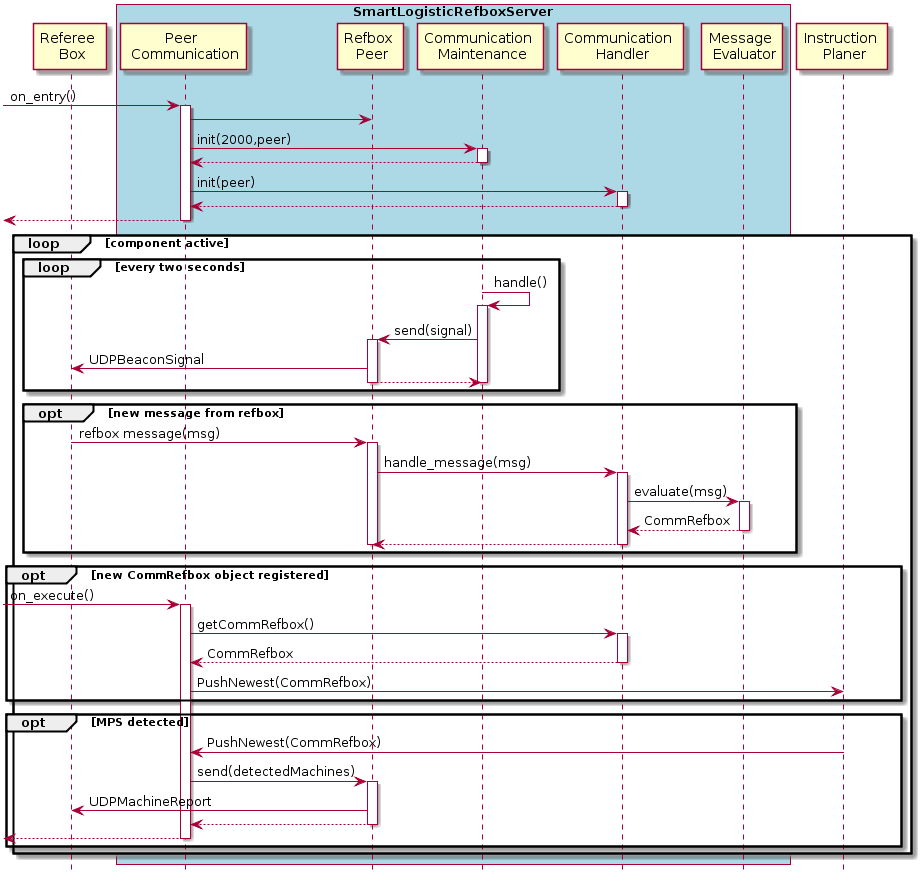
\includegraphics[width=\linewidth]{pic/sequence_diagram_RefboxServer.png}
\caption{Sequence diagram of Refbox server \cite{BOK}}
\label{fig:sequenceDiagramRefboxServer}
\end{figure}


\subsubsection{Difficulties}

On the Refbox server, the encryption was different during the competition and in the laboratory. An Electronic Code Book (ECB) encryption was needed in Robocup and Cipher Block Chaining (CBC) encryption is used with the Refbox installed in the laboratory. \\